\label{ch:introduction}
\section{Overview}
In this thesis, we present a model using deep inverse reinforcement learning that aims to capture and replicate the art of moving through densely populated spaces in a socially acceptable manner. \edited{A style of navigation can be said socially acceptable if it does not draw unwanted attention from nearby humans. Conditions that aid in the cause include but are not limited to respecting personal spaces while not being overtly cautious, maintaining basic decorum e.g. not cutting off others or moving through groups who are interacting with each other, and following social norms e.g. keeping to the right while moving through a narrow passage}.\\
Society is diving headfirst towards a future where humans and machines coexist. \edited{Robots come in all shapes, sizes and use-cases, but here we concentrate specifically on mobile (service) robots that interact with humans while operating in close proximity.}. Robots have been deployed in the vicinity of humans since as early as 1998, when Nourbaksh et al. installed a tour guide robot Mobot as a permanent member of the Carnegie Museum of Natural History for 5 years, till 2002 \cite{Nourbaksh2003Movot}. \edited{Other notable examples of interactive mobile robots}: Robox, \cite{siciliano_robox_2003} which was deployed for 157 days at the Swiss international exhibition in 2002 where it was assigned the task of giving tours, taking pictures, and providing entertainment to the visitors, Minerva \cite{minerva_thrun_2000}, deployed in 1998 at the Smithsonian Museum of American History again as a tour guide for 14 days, Rhino \cite{fox_dynamic_1997}, deployed at the Deutsches Museum Bonn for 6 days in 1997, Rackham \cite{rackham_clodic_2006} and CiceRobot \cite{chella_perception_2009} both of which served the role of a tour guide at a museum.\\
%\\Pictures of robots that have been deployed in the real world.
\vspace{3cm}
\begin{figure}
	\label{fig:real-world-robots}
	\centering
	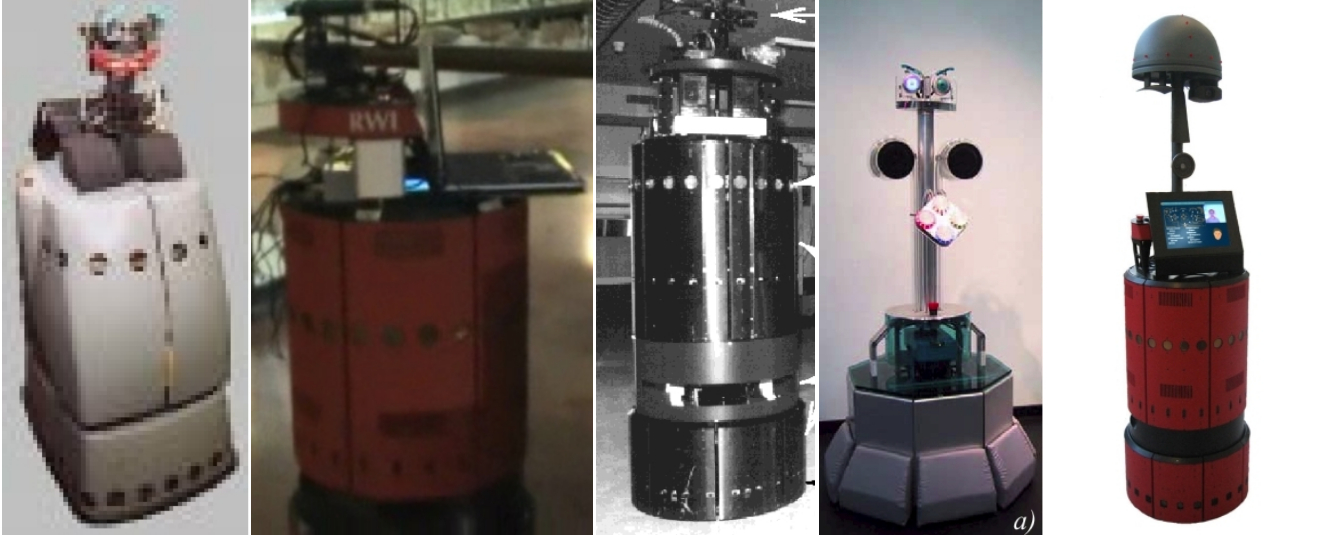
\includegraphics[width=\linewidth]{figures/minerva_cice_rhino_robox_rackham.jpg}
	\caption{Some robots that have been deployed in the real world. From the left to right: Minerva, CiceRobot, Rhino, Robox and Rackham.}
\end{figure}

Other than guiding people in museums and exhibitions, mobile robots have also been deployed in the field of healthcare: \cite{pearl_pollack_2002}, \cite{kim_socially_2016}, and \cite{kuderer_feature-based_nodate} and shopping malls: Shopbot \cite{shopbot_kanada} and Toomas \cite{toomas_gross_2009} who provided interactive support and guidance to people. 

%With some of the more recent works done by Kim and Pineau and Kretzschmar et al take a different approach. Instead of working with helper robots to guide others, the choose robotic wheelchairs as their platform to help disabled individuals navigate through human crowds. \\

%Today, we are surrounded by machines of varying complexity, competence, and autonomy, all with the common goal of making human life easier. Some common use cases include but are not limited to: giving museum tours, guiding people at the airport, assisting the elderly and needful.   \\

Navigation is one of the fundamental problems in the field of mobile robotics with decades of research flowing into it. In its simplest form, it can be defined as a process that enables a robot to move from its current position (stating position) to a desired position( goal position) avoiding collisions along the way. Work on artificial potential field by O.Khatib \cite{khatib_1986} and various flavors of graph-based search algorithms address this problem. \edited{In terms of deployment in the real world, Shakey Project \cite{project-shakey} was among the first to introduce a robot with capabilities to successfully perceive and navigate its surroundings.}\\

Deploying mobile robots in the presence of humans introduces a new set of challenges. Avoiding collisions and reaching a given destination are no longer sufficient, now these must be achieved in a 'socially acceptable' manner. The \edited{subjective} nature of this additional objective of being socially acceptable makes the problem \edited{especially} challenging. This is primarily because there is no strict definition of 'socially acceptable', and is highly dependent on the socio-cultural background of the people in the crowd and the situation at hand. This warrants and subsequently has led to research specifically geared towards socially compliant navigation.\\

\thcomment{"Even though navigation is a basic robot skill, the robotics and HRI communities have not yet produced
	a holistic approach to human-aware navigation. However, pioneering works on several individual aspects
	of human-aware navigation exist. This paper introduces human-aware navigation as a research topic and
	provides an overview of the existing research, including not only navigation techniques, but also evaluation
	methods." - \cite{kruse_human-aware_2013}\\ Can I use this to cite for the statement "This warrants and subsequently has led to research specifically geared towards socially compliant navigation."}

\edited{Kruse et. al. \cite{kruse_human-aware_2013} identify 3 broad areas of focus in the existing literature that make a robot more acceptable in a social context, which leads to improvement in $3$ qualitative attributes:}

\thcomment{ From what I have found so far, \cite{kruse_human-aware_2013} is one of the most cited survey paper on this topic in recent times.}
\begin{enumerate}
    \item \textbf{Comfort}: how comfortable people are around a robot. 
    \item \textbf{Naturalness}: how natural the movement of a robot is. This is synonymous with the predictability and interpretability of the robot's movements.
    \item \textbf{Sociability}: respecting cultural norms like preferring the right side of a hallway and, not cutting through a group of people: to name a few. %These fall into the category of what we like to call 'common courtesy'
\end{enumerate}

\subsubsection{Work on comfort}
Addressing the aspect of comfort has been one of the more researched areas in the field of social navigation \cite{kruse_human-aware_2013}.\\

\thcomment{"Research on human-aware robot navigation follows different goal: \textbf{Most of the papers we collected attempted to minimize annoyance and stress, thus making interaction more comfortable for the human.} Others
	strive to make robots behave more natural within their abilities or make robots behave according to cultural
	norms. All three goals have in common that they attempt to improve robot acceptance, but the methods
	vary. These terms like "comfort" and "natural" are used loosely in literature, so in order to classify the
	papers, we use the following definitions." - \cite{kruse_human-aware_2013}}

 Relative distance from a person has been the primary gauge to measure comfort. These are largely based on the work of Edward T. Hall in proxemics \cite{proxemics_hall_1968}. Proxemics deals with the study of personal territory. While this is dependent on the socio-cultural background of an individual, and the context of the scene, Hall divides the personal territory into 4 \edited{zones}: public, social, personal, and intimate, each reserved for a different purpose as described in \autoref{tab:proxemics}
\begin{table}
    \begin{center}
        \renewcommand{\arraystretch}{1.3}
        \begin{tabular}{|p{0.2\textwidth}|p{0.15\textwidth}|p{.57\textwidth}|}
            \hline
            Name of zone & Distance & Use case \\
            \hline\hline
            Intimate space & 0 - 45cm &  Interacting with close friends and intimates. Generally involving physical contact.\\
            Personal space & 45 -120cm &  For interaction with close friends and family. \\
            Social space & 1.2 - 3.6m &  Interacting with acquaintances and people one is familiar with.\\
            Public space & > 3.6m &  Interacting with a crowd of people.\\
            \hline
        \end{tabular}
        \caption{Categorization of Proxemic distances.}
        \label{tab:proxemics}
    \end{center}
\end{table}
Other work exploring the comfort aspect of human-robot communication focuses on specific cases like:
\begin{enumerate}
    \item \textbf{Approaching a person:} Dautenhahn et al. \cite{dautenhahn_2006}  study different ways to approach people who are seated. They find that the best way is to approach from the side and not from the front.
    [Koay et al. \cite{koay2007ExploratorySO}  found that $58\%$ of participants preferred a frontal approach by the robot while $75\%$ preferred a frontal approach when the robot was handing them something.
    \item \textbf{Passing a person:} [Pacchierotti et al. \cite{pacchierotti_2006} \cite{pacchierotti_2005},  show that proper signaling while approaching a person and maintaining a healthy distance is a desired trait in a mobile robot.
    \item \textbf{Moving in the vicinity of a person:}  Butler et al. \cite{butler_2001} test on different approaching speeds, trajectories taken by a robot to avoid a person and exploratory movements of robots in general and find that in general people prefer slower speed, and greater gap maintained by a robot passing by.
\end{enumerate}

\edited{A majority of the existing work, that aim to increase comfort, design cost-maps based on the findings of the aforementioned studies.} These produce navigating agents that maintain a healthy distance from nearby people. Some aim to reduce the surprise factor in their robot navigation by structuring penalty functions that emphasize motion in the field of view of nearby people \cite{pandey_2010_human_centered_nav}, \cite{scandolo_2011}, \cite{sisbot_human_2007}.
Others concentrate on specific scenarios like approaching, tracking, and following people.\\

Recent works using reinforcement learning algorithms also fall into this category. They primarily focus on two things: the structure of the reward, and the representation of the environment. \\

Rewards are engineered focusing on collision avoidance and maintaining proxemics distances from nearby pedestrians \cite{chen_crowd_aware_robot_nav_with_attention}, \cite{chen_decentralized_non_communication_2017}. Other works incorporate a more intricately designed reward function that captures rudimentary social norms like overtaking from the left,  and passing from the right \cite{chen_socially_2017}. \\
\thcomment{\cite{chen_socially_2017} is a work on robots interacting with pedestrians. I am guessing people follow similar rules while walking?}

\edited{Reinforcement learning algorithms base their decisions on observations from the environment. A key component of these methods is the precise interpretation and proper representation of its nearby surroundings to generate meaningful observations. Long et al. \cite{long_2017_optimally_decentralized_collision_avoidance} and Tai et al. , \cite{tai_paolo_virtual_to_real_2017} work with raw observations from the environment. Chen et al. use pairwise interaction \cite{chen_crowd_aware_robot_nav_with_attention}, \cite{chen_decentralized_non_communication_2017} between a robot and the pedestrians nearby, modeling human-human interaction using local maps \cite{chen_crowd_aware_robot_nav_with_attention}, and pooling information using attention-based mechanisms \cite{chen_crowd_aware_robot_nav_with_attention}.}

\subsubsection{Work on naturalness}
\edited{While comfort is necessary, it is not sufficient.} Naturalness in the motion of the robot and the trajectory it traces play an important role in the social acceptance of a robot. \\
\thcomment{This is all I have regarding this : "Several publications attempt to make robots navigate more acceptably near humans by making robots
	move more similar to how humans move. This is often called "natural" behavior. The assumption is that if a
	robot behaves like a human (or like an animal), the interaction between humans and the robot becomes easier
	and more intuitive for the humans. Related adjectives are "predictable", "understandable", "readable" or
	"legible". All those concepts rely on the fact that robot motion is interpreted by human observers, who
	attempt to judge the motive and the future behavior of the robot. As an example this is necessary as a
	human might need to proactively interrupt the robot if the safety of the human, the robot or the environment
	are at risk. The likelihood that a human observer interprets the motion of the robot correctly is assumed
	to be higher if the robot moves naturally." - \cite{kruse_human-aware_2013}. So, I think it is more of an assumption than hard evidence.}
\\Work falling under this category deal with the motion of the robot, rather than its effect on its surrounding and attempts to improve its predictability and interpretability.\\ %If a human being sees the robot, he/she would be able to understand/interpret its intentions and the trajectories taken by the robot would somewhat be similar to that of a person put in a similar context. 
Factors that help perceive a mobile robot as natural include:
\begin{enumerate}
    \item \textbf{Smooth motion:} Humans prefer a gradual, consistent change in orientation and velocity. This traces smooth paths that optimize for the energy spent in the execution of the trajectory \cite{arechavaleta_nonholonomic_2008}. Sudden changes in orientation and speed while moving in a crowd makes a robot unpredictable and thus seem unnatural. \cite{pandey_alami_robot_guide_2009, pandey_2010_human_centered_nav} work on smoothing trajectories.
    \item \textbf{Natural interaction:} A large portion of the time we spend during navigation in groups involves interaction with others. Some of the traits we commonly exhibit that has been the focus of research are following people moving in the general desired direction \cite{gockley_natural_person_following_2007}, maintaining a formation while interacting with nearby people \cite{althaus_nav_for_human_robot_interaction_2004}, and non-verbal communication with people nearby \cite{sauliner_minimal_nonverbal_interruption_2011}. 
    
\end{enumerate}
\thcomment{Figure for the above if possible}
\subsubsection{Work on sociability}
Social and cultural norms are the collection of explicit and tacit rules that we as a member of the society agree up to maintain harmony. Examples of this would include but not limited to waiting in a queue, preferring a particular side of a pathway, and waiting for people to exit an elevator before entering. While the presence of these traits is not vital, the lack of adherence to social norms can cause discomfort and evoke mistrust among people nearby. Some of the work in the existing literature addresses a few of these problems. Kirby et al. \cite{kriby_companion_2009} encodes within their cost function the preference for the right side of a corridor. \cite{pandey_alami_robot_guide_2009} make the robot overtake a pedestrian from the right.\\

While most of the approaches produce reliable controllers on and off the simulator, they optimize for a set of goals that are geared towards optimizing for navigation using a smartly engineered reward function which in turn relies on proxemic distances and in some cases a few of the obvious social norms.\\

\section{Inverse reinforcement learning in social navigation}
One of the primary issues associated with formulating a reward function for social navigation is the vast variety and elusiveness of the 'social rules'. \edited{Inverse reinforcement learning (IRL) or inverse optimal control is a class of methods} put forward by Russell \cite{russel_irl_1998} that seek to address this issue. \edited{The goal of IRL is to recover the underlying reward function and use it to obtain an optimal controller. This is achieved by optimizing the reward function to maximize the likelihood of the expert demonstrations.}\\
\edited{Abbeel and Ng \cite{abbeel_apprenticeshiplearning_2004} show a positive correlation between match in feature expectation of the agent and the expert to similarity in their performance in the context of a Markov decision process(MDP).}
Abbeel and Ng \cite{abbeel_apprenticeshiplearning_2004} show that matching the feature expectation of the agent to that of the expert equates to a similarity in their performance in the context of a Markov decision process(MDP). But the problem remains under constrained as multiple reward functions (including degenerate ones) can lead to the expert demonstrations being optimal. Additionally, the idea of feature matching is ambiguous, as a single policy can be optimal for different reward functions and different policies can lead to similar feature expectations. \\

Ziebart et al. \cite{ziebart_maxent_2008} takes an entropy-based approach to resolve this ambiguity. They use an energy-based model where the probability of a given trajectory is proportional to the exponential of the reward it obtains.
\thcomment{These will be explained in greater details later.}
This produces stochastic policies that have equal preference over trajectories yielding similar rewards. Recent developments in IRL introduce the use of neural networks bolstering the expressive power of the reward function \cite{wulfmeier2015maximum}. \\

\edited{Diversity in socio-cultural norms makes the defining concrete rules for social navigation difficult, as a consequence, IRL has been heavily explored in this field \cite{kuderer_socially_nodate, kretzschmar_socially_2016}.} \cite{shiarlis_rapidly_2017, okal_efcient_nodate} use IRL in conjunction with more traditional graph-based navigation methods to train agents. They use the IRL to infer the underlying rewards, which are then used to estimate the cost of different paths. Kim et al. \cite{kim_socially_2016} use IRL in a hierarchical navigation architecture, where they divide the task of navigation into a long term global planner based on a classical shortest-path algorithm, a short term controller based on IRL and a low-level collision avoidance module. \cite{kretzschmar_socially_2016} use a spline-based representation of the trajectory and use a maxent IRL formulation to train an agent using feature matching. 
\\
Both,\cite{kim_socially_2016, kretzschmar_socially_2016} implement their method on real-world robots. \cite{vasquez_inverse_2014} provide a comparative analysis of different IRL based learning algorithms and the importance of feature representation in the context of IRL. More recent works include deep learning-based methods to solve the problem of social navigation \cite{fahad_learning_2018, wulfmeier2015maximum}


\edited{In this thesis, we propose an efficient sampling-based approximation of the state visitation frequency of the agent. This permits our method to work even in environments that do not have well-defined state dynamics. This is particularly useful in real-world applications. We also propose a feature representation for the social-navigation problem that captures relevant information from the environment. The feature representation in conjunction with the proposed method generates agents that exhibit improved navigational performance compared to existing work.}

%sampling based SVF calculation for model-free environment. 
%New feature representation to go along with it.

\section{Thesis outline}
The rest of the chapters of the thesis are organized as follows:
\autoref{ch:2} and \autoref{ch:3} present a detailed overview of some of the existing work in the literature based on both classical methods and data-driven approaches respectively.

\autoref{Ch:4} elaborates on the proposed navigation pipeline describing a flavor of the MEDIRL algorithm for a model-free environment along and design and the idea behind the design of the feature representation used.

We train and test our methods in an in-house built simulator, specifically designed for the task of social navigation, which is described in great detail in \autoref{ch:enviornment}

%is dedicated to the experiments performed, the metrics used to measure their performance and finally a detailed analysis of the results obtained and how they compare to the existing work.
\edited{\autoref{ch:6} contains details about the different experiments conducted and how the different components of the navigation algorithm, like the feature representation and the choice of the training algorithm, contribute to the final performance of the agent. Measuring the social compliance of an agent can be tricky. Keeping that in mind, we introduce a set of evaluation metrics, both subjective and objective in this chapter. Lastly, we present a detailed analysis and subsequent evaluation of the results obtained and the contribution of the different components towards it.}

\autoref{ch:conclusion} concludes the thesis reflecting upon the challenges faced in the task of social navigation and includes possible avenues to explore building upon the existing work.
